%%% ---------------
%%% PREAMBLE
%%% ---------------
\documentclass[french,11pt,a4paper]{article}

% Define geometry (without using the geometry package)
\usepackage{geometry}
\geometry{landscape, twocolumn, textwidth=27.5cm, textheight=19.5cm, columnsep=15mm}

%\frenchspacing						% better looking spacing

% Call packages we'll need
\usepackage{graphicx}				% images
\usepackage{amssymb,amsmath}		% math
\usepackage{multicol}				% three-column layout
\usepackage{multirow}
\usepackage{url}					% clickable links
\usepackage{marvosym}				% symbols
\usepackage{wrapfig}				% wrapping text around figures
\usepackage{fontspec}			% font encoding
\usepackage{xunicode}
\usepackage{ragged2e}
\usepackage{titlesec}
\usepackage{framed}
%\usepackage[default]{raleway}
\usepackage{tocvsec2}
% Customize (header and) footer
\usepackage{fancyhdr}
\usepackage{enumitem}
\usepackage{fontawesome}
\usepackage{lipsum}
\usepackage{babel}
%\pagestyle{fancy}
\pagestyle{empty}
\setmainfont{Carlito}

%\titlespacing\section{0pt}{0pt plus 4pt minus 2pt}{0pt plus 2pt minus 2pt}
%\titlespacing\subsection{0pt}{12pt plus 4pt minus 2pt}{0pt plus 2pt minus 2pt}
%\titlespacing\subsubsection{0pt}{12pt plus 4pt minus 2pt}{0pt plus 2pt minus 2pt}

%\newfontfamily\headingfont[]{Arial}
%\titleformat*{\section}{\Large\bfseries\sffamily}
%\titleformat*{\section}{\Large\headingfont}

%\renewcommand{\headrulewidth}{0.0pt}	% no bar on top of page
%\renewcommand{\footrulewidth}{0.4pt}	% bar on bottom of page

%%% ---------------
%%% DEFINITIONS
%%% ---------------

% Define separators
\newcommand{\HorRule}[1]{\noindent\rule{\linewidth}{#1}} % Creating a horizontal rule
\newcommand{\SepRule}{\noindent							 % Creating a separator
						\begin{center}
							\rule{250pt}{1pt}
						\end{center}
						}						

% Define Title en News input
\newcommand{\JournalName}[1]{%
		\begin{center}	
			%\Huge \usefont{T1}{augie}{m}{n}
            \Large \usefont{T1}{augie}{m}{n}
			#1%
		\end{center}	
		\par \normalsize \normalfont}
		
\newcommand{\JournalIssue}[1]{%
		\hfill \textsc{\mydate \today, No #1}
		\par \normalsize \normalfont}
\newcommand*{\chants}{../chants}
\newcommand*{\messe}{../messe_bienveillance}
\newcommand*{\pu}{../pu}
\newcommand*{\psaumes}{../psaumes}
\newcommand*{\footer}{..}

\newcommand{\NewsItem}[1]{%
\vspace{3pt}
\underline{\textbf{#1}}
	%	%\usefont{T1}{augie}{m}{n} 	
	%	\large \textbf{#1} %\vspace{3pt}
   %     %\Large #1 \vspace{4pt}
	%	%\par 
   %     \normalsize \normalfont
		  }
		
\newcommand{\NewsAuthor}[1]{%
			\hfill by \textsc{#1} \vspace{4pt}
			\par \normalfont}		

\graphicspath{{../images/}}

%pas de numérotation des sections
\setsecnumdepth{none}
\setlength{\parindent}{0pt}
%%% ---------------
%%% BEGIN DOCUMENT
%%% ---------------
\begin{document}

\NewsItem{CHANT D'ENTRÉE}
	\textbf{Jubilez criez de joie}

Jubilez, criez de joie. Acclamez le Dieu trois fois Saint ! Venez le prier dans la paix, témoigner de son amour.
Jubilez, criez de joie pour Dieu notre Dieu.

1 - Louez le Dieu de lumière. Il nous arrache aux ténèbres. Devenez en sa clarté des enfants de la lumière.

5 - Louange au Père et au Fils, louange à l'Esprit de gloire. Bienheureuse Trinité, notre joie et notre vie !


\NewsItem{PRÉPARATION PÉNITENTIELLE} \\
	Seigneur, prends pitié. Seigneur prends pitié, Seigneur, prends pitié\\
Ô Christ, prends pitié. ô Christ prends pitié, o Christ, prends pitié.\\
Seigneur, prends pitié. Seigneur, prends pitié Seigneur, prends pitié


\NewsItem{GLORIA}
	\begin{itemize}
\item[R/] 
Gloire à Dieu, au plus haut des cieux, et paix sur la terre, aux hommes qu'il aime. (bis)
\item[1.]
Nous te louons, nous te bénissons, nous t’adorons, nous te glorifions, nous   
      te rendons grâce pour ton immense gloire. Seigneur Dieu, Roi du ciel, Dieu 
      le Père tout puissant. R/
\item[2.]
Jésus-Christ, Seigneur Fils unique, Agneau de Dieu, le Fils du Père, toi qui 
      enlèves le péché du monde, reçois nos prières. Toi qui es assis à la droite  
      du Père, prends pitié de nous. R/
\item[3.]
Car toi seul es saint, toi seul es Seigneur, toi seul es le Très Haut : 
      Jésus-Christ, avec le Saint Esprit, dans la gloire de Dieu le Père. R/
\end{itemize}




% -----
\NewsItem{1\iere{} LECTURE} Pr 8, 22-31
% -----

\NewsItem{PSAUME}
Ps 8, 4-5, 6-7, 8-9

\textbf{
Ô Seigneur, notre Dieu,
qu’il est grand, ton nom,
par toute la terre !
}

À voir ton ciel, ouvrage de tes doigts,
la lune et les étoiles que tu fixas,
qu’est-ce que l’homme pour que tu penses à lui,
le fils d’un homme, que tu en prennes souci ?

Tu l’as voulu un peu moindre qu’un dieu,
le couronnant de gloire et d’honneur ;
tu l’établis sur les œuvres de tes mains,
tu mets toute chose à ses pieds.

Les troupeaux de bœufs et de brebis,
et même les bêtes sauvages,
les oiseaux du ciel et les poissons de la mer,
tout ce qui va son chemin dans les eaux.


% -----
\NewsItem{2\ieme{} LECTURE} Rm 5, 1-5

\NewsItem{ACCLAMATION}
%Alleluia \emph{messe du Peuple de Dieu}


\NewsItem{ÉVANGILE} Jn 16, 12-15

\NewsItem{HOMÉLIE}

\NewsItem{PROFESSION DE FOI}

%\newpage

\NewsItem{PRIÈRES UNIVERSELLES} 
Ô seigneur envoie ton esprit qui renouvelle la face de la terre.


\NewsItem{OFFERTOIRE}

\NewsItem{PRIÈRES SUR LES OFFRANDES}
\textit{Nous nous levons et nous répondons : }
Que le Seigneur reçoive de vos mains ce sacrifice à la louange et à la gloire 
de Son nom, pour notre bien et celui de toute l’Église.

\NewsItem{SANCTUS}
Le Seigneur est Saint ! Le Seigneur est Saint ! Le Seigneur est Saint !
Le Seigneur est notre Dieu, Le Seigneur est notre Père. Il règne dans les cieux, qu’Il règne sur la terre.


\NewsItem{ANAMNÈSE}
Christ est venu, Christ est né, Christ a souffert, Christ est mort, 
Christ est ressuscité, Christ est vivant,
Christ reviendra, Christ est là,
Christ reviendra, Christ est là.


\NewsItem{NOTRE PÈRE}

\NewsItem{AGNUS} \\
Agneau de Dieu Qui enlèves le péché du monde, Prends pitié de nous !  Prends pitié de nous ! (bis) \\
Agneau de Dieu Qui enlèves le péché du monde, Donne-nous la paix !  Donne-nous la paix !


\NewsItem{COMMUNION}
\textbf{La sagesse a dressé une table}

\textbf{
La sagesse a dressé une table,
Elle invite les hommes au festin.
Venez au banquet du fils de l'homme,
Mangez et buvez la Pâque de Dieu.
}

1.
Je bénirai le Seigneur en tout temps,
Sa louange est sans cesse à mes lèvres.
En Dieu mon âme trouve sa gloire,
Que les pauvres m'entendent et soient en fête !

2.
Proclamez avec moi que le Seigneur est grand,
Exaltons tous ensemble son nom !
J'ai cherché le Seigneur et il m'a répondu
De toutes mes terreurs il m'a délivré.

3.
Tournez vous vers le Seigneur et vous serez illuminés
Votre visage ne sera pas couvert de honte ;
Un pauvre a crié, et Dieu a entendu,
Le Seigneur l'a sauvé de toutes ses angoisses.

%4.
%L'ange du Seigneur a établi son camp,
%Il entoure et délivre ceux qui le craignent.
%Goûtez et voyez que le Seigneur est doux,
%Bienheureux l'homme qui trouve en lui son abri !


\NewsItem{CHANT D'ENVOI}
\textbf{Prenons la main}

1. Prenons la main que Dieu nous tend.
Voici le temps, le temps où Dieu fait grâce à notre terre.\\
Jésus est mort un jour du temps.
Voici le temps, le temps de rendre grâce à notre Père.\\
L´unique Esprit bénit ce temps.
Prenons le temps, le temps de vivre en grâce avec nos frères.

2. Prenons la paix qui vient de Dieu.
Voici le temps, le temps où Dieu fait grâce à notre terre.\\
Jésus est mort pour notre vie.
Voici le temps, le temps de rendre grâce à notre Père.\\
Son règne est là : le feu a pris.
Prenons le temps, le temps de vivre en grâce avec nos frères.



\newpage


\NewsItem{Intentions de messe (Sainte Croix)}
\begin{itemize}
\item[\Cross]
Raymond MAIER et Marie Claire NOËL
\item[\Cross]
Les âmes du purgatoire de la famille GENNETAY
\end{itemize}

\NewsItem{Informations paroissiales}

\begin{tabular} {lcp{9cm}}
\multicolumn{3}{c}{\textbf{Saint Jean-Baptiste} } \\ \hline
Mardi    & 17 juin  & Vêpres 18h15. Messe 18h30 \\ \hline
Jeudi    & 19 juin  & 
Exposition du Saint Sacrement à 16h00. Adoration. Salut au Saint Sacrement à 18h15. Messe à 18h30 
 \\ \hline
Vendredi & 20 juin  & Laudes 08h45. Messe 09h00 \\ \hline
Samedi   & 21 juin  & Messe anticipée 18h00 \\ \hline
Dimanche & 22 juin  & \emph{Le Saint Sacrement du corps et du sang du Christ}
\mbox{\textbf{Procession}} 09h30 \textbf{Messe} 10h00\\ \hline
\multicolumn{3}{c}{\textbf{Sainte Croix} } \\ \hline
Mercredi & 18 juin  & Messe 09h00.
%\newline \Cross{} \textbf{Enterrement}  14h30 Marie-Claire Noël 
\\ \hline
Dimanche  & 22 juin  & Pas de messe\\ \hline
%\multicolumn{3}{c}{\textbf{Résidence Landsberg (3 rue Jean Monnet)} } \\ \hline
%Mercredi & 04 juin : & Messe 10h45 \\ \hline
\end{tabular}

\begin{framed}
\begin{tabular} {lcp{8cm}}
\multicolumn{3}{c}{\textbf{Saint Jean-Baptiste} } \\
Dimanche & 15 juin  & 17h00 Concert \og Haut en couleurs \fg avec l'ensemble vocal \textbf{Diapason}. Prix libre. \\
%\multicolumn{3}{c}{\textbf{Foyer Oberlin} } \\
%Vendredi & 13 juin  & 20h00 - 21h00 \textbf{Nuit des veilleurs}. Venez prier avec l'ACAT pour les victimes des persécutions.
\end{tabular}
\end{framed}


\NewsItem{Répétitions des chorales}
\begin{description}
\item[Chorales paroissiales] : reprise le vendredi 05 septembre (20h15 à Ste Croix)
%\item[Chorales paroissiales] : vendredi 20h15 à Sainte Croix
\end{description}

\begin{framed}
\textbf{Presbytère St Jean-Baptiste}
%2 rue de l'école 67380 Lingolsheim 03 88 78 16 45 \\
2 rue de l'école 67380 Lingolsheim \phonenumber[country=FR]{0388781645} \\
\textbf{Permanence} Lun. au Jeu. : 09h30-12h00 et 15h-18h. Ven. 16h-18h00. Sam. 09h30-12h00. \\
\textbf{Courriels} \texttt{nddessables@hotmail.com}, \texttt{danielette67380@gmail.com}

%\textbf{Caritas} Vestiaire ouvert le mardi de 14h à 16h

\texttt{https://stjeanbaptistelingo.fr} \hfill \faFacebook Catho Lingo \hfill \faInstagram @catho\_lingo
\end{framed}



\newpage

\JournalName{Communauté de Paroisses de Lingolsheim \\
\normalsize \textit{Notre Dame des Sables}
%\\ \large \'{E}glise Saint Jean-Baptiste
\\  \normalsize \textit{Sainte Trinité}
\\ \large Dimanche 15 juin  2025}
%\noindent\HorRule{3pt} \\[-0.75\baselineskip]
%\HorRule{1pt}
% -----

% Front article
% -----
%\vspace{0.5cm}
%	\SepRule
%\vspace{0.5cm}

%\begin{center}
\begin{minipage}[h]{1.0\linewidth}
% \begin{center}
 \textbf{
 %\dots
\og 
Rentrée Pastorale 2025-2026
 \fg{}
 %\dots
 }
 \end{center}

%\begin{wrapfigure}{l}{1.3cm}
%\vspace{-0.4cm}
%	\includegraphics[scale=1.0]{../images/lazarre}
%\end{wrapfigure}
Une nouvelle rentrée pastorale qui nous réjouit tous. En effet, après un temps de répit, il nous revient de mettre en marche la machine de nos activités pastorales.

Au début de cette nouvelle année pastorale, je souhaite vous redire toute ma joie de vous retrouver pour continuer la mission qui m’est assignée dans notre communauté de paroisses. Et comme chaque année, nous mettrons l’accent en premier lieu sur la vie catéchétique des enfants et des adolescences, l’animation liturgique, la création d’une troisième chorale, la visite aux malades et dans notre maison de retraite ( \emph{Résidence du Parc}), l’accueil et l’accompagnement en vue de baptêmes,  du catéchuménat des adultes, des mariages, l’encadrement  des servants d’autel, l’entretien de notre église pour la rendre  accueillante, avec ces innombrables petits gestes de service qui jalonnent l’existence ; tout cela nous aidera à vivre une véritable dimension ecclésiale.

Je voudrais vous remercier de tout cœur, vous tous qui êtes des membres vivants et actifs de la communauté paroissiale que nous formons, véritable artisans de l’évangélisation ordinaire. Mon souhait pour la vie de notre communauté de paroisses est que nous arrivions toujours plus à nous ouvrir et à nous connaître les uns les autres, à nous apprécier dans ce que nous sommes et vivons.

L’année dernière, avec toutes les entités de nos deux paroisses, nous avons eu différentes propositions, activités et invitations qui ont favorisées l’\textbf{Unité et l’ouverture} qui constituaient notre thème pastoral. Ne manquons pas cette année ces moments simples et conviviaux qui permettent de tisser des liens gratuits, profonds et tout simplement chrétiens.

\begin{wrapfigure}{l}{1.2cm}
\vspace{-0.4cm}
	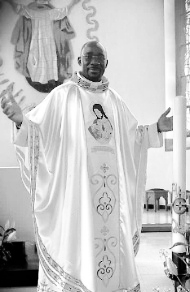
\includegraphics[scale=1.20]{../images/standing_daniel}
\end{wrapfigure}
Cette année nous porterons ensemble cette rentrée dans le cœur de chacun avec nos \textbf{jeunes pro}. Chacun à son rythme, selon ses possibilités et ses réalités mais avec un seul et même objectif : l’accomplissement de nos activités communautaires. Présentons également notre rentrée paroissiale au Christ. Et continuons notre chemin pour la mise en œuvre de notre projet paroissial autour de ce principal thème : \textbf{\og Avec notre jeunesse bâtissons une communauté plus dynamique, rayonnante et missionnaire\fg{}.}

	Que cette rentrée pastorale nous aide à prendre des résolutions nécessairement pour plonger à frais nouveaux dans la parole et être des disciples crédibles de l’évangile.


\begin{flushright}
Bonne rentrée pastorale à toutes et à tous !
\textit{Père  Daniel  ETTÉ}
\end{flushright}


\lipsum[1-3]
\end{minipage}
%\end{center}
% -----
\end{document} 
